% !TeX spellcheck = en_GB
\documentclass[a4paper,12pt]{article}

\usepackage{anysize}
\marginsize{30mm}{20mm}{20mm}{20mm}
\usepackage[utf8]{inputenc}
%\usepackage[english]{babel}
\usepackage[style=ieee,backend=biber,url=false,isbn=false]{biblatex}
\usepackage[final]{microtype}
\addbibresource{LitReview.bib}
\usepackage{amsmath}
\usepackage{graphicx}
\graphicspath{ {./images/} }
\usepackage{setspace}
\singlespacing
\usepackage{gensymb}
\parskip 0ex
\usepackage{array}
\newcolumntype{D}{>{\centering\arraybackslash}m{0.65\textwidth}}
\newcolumntype{L}{>{\centering\arraybackslash}m{0.45\textwidth}}
\newcolumntype{M}{>{\centering\arraybackslash}m{0.3\textwidth}}
\newcolumntype{S}{>{\centering\arraybackslash}m{0.195\textwidth}}
\newcolumntype{V}{>{\centering\arraybackslash}m{0.095\textwidth}}

%opening
\title{Literature Review \\
	\large Linear Direct Current Electromagnetic Motor with\\
	Liquid Eutectic Gallium-Indium Alloy Coil}
\author{Jason Guan}
\begin{document}
\maketitle
\begin{center}
    892594255\\
    Department of Engineering Science\\
    Supervised by Dr. Bryan Ruddy
\end{center}
\thispagestyle{empty}

\newpage

\section{Introduction and Background}

Soft robots are the next frontier in robotics. Traditional robots rely on rigid materials for actuation. Rigid designs can be easily and precisely predictable, making them easier to design and manufacture. However, these benefits come at a cost. Rigid designs have narrow ranges of operating conditions, are suspectable to wear and fatigue, and tend to be less human friendly \cite{rusDesignFabricationControl2015}.

Over the last two decades, research has turned to the possibility of robots and actuators made with mechanically compliant materials. The promise of soft robots is that they would be adaptable in unpredictable conditions, and comfortable for wearable use \cite{leeSoftRobotReview2017}. Research in soft robot actuation has mostly focused on chemical\cite{onalSoftMobileRobots2017}, pressure-based (pneumatic or hydraulic)\cite{suzumoriBendingPneumaticRubber2007} and electroactive elastomer\cite{andersonMultifunctionalDielectricElastomer2012} methods. Electromagnetic actuation that most traditional robots rely on has been relatively overlooked and gained interest only over the past 4 years. Jin et al. published \cite{jinStretchableLoudspeakerUsing2015} in 2015, one of the first studies that explored electromagnetic actuation in soft designs. Jin et al. introduced a voice coil speaker that is effective under large deformations. Electromagnetic actuation is well-studied in rigid systems, and the knowledge may be transferable to soft robots.

Cooling is another challenge in actuator design regardless of flexibility. This is an especially large problem for electromagnetic actuators, where heating is uniform but cooling is more efficient closer to the surface. This has prompted the development of several innovative solutions such as direct liquid cooling \cite{henkeChallengesOpportunitiesVery2018}. However, all of these methods require advanced manufacturing techniques and tightly controlled conditions, rendering them expensive and inflexible. Furthermore, none of these methods are transferable to soft robots.

Therefore, there is a need for developing electromagnetic actuation methods for soft robots, and cooling methods for those actuators.

\section{Materials}

\subsection{Highly Deformable Materials}
Soft robots are made possible by the increasing availability of highly compliant yet tough materials. These materials tend to fit in the categories of rubbers, elastomers, polymers and polymer composites. Silicones, a type of synthetic polymer, are known to be the most suitable materials available for most soft robot construction. This is due to silicones’ low elastic moduli, high resilience and toughness, ability to actuate over millions of cycles and rich body of literature \cite{polygerinosSoftRoboticsReview2017}. A review of literature found no published soft robot research designs that did not involve silicones in some way. Some designs used a combination of soft and hard components \cite{stokesHybridCombiningHard2013} or silicone composites \cite{laschiSoftRobotArm2012}.

\subsection{Gallium-Indium Eutectic Alloy}
A large challenge that prevented the use of electromagnetic actuation in soft designs was the lack of good conductors that maintain their properties under large deformations. Older approaches such as conductive silicone rubber seen in Figure \ref{fg:conductiveRubber}, have non-linearly varying electrical properties under deformation \cite{valentaMechanicalElectricalTesting2008}. The silicone rubber also has poor conductivity, with resistance several magnitudes higher than conventional conductors.

\begin{figure}[h!]
    \centering
    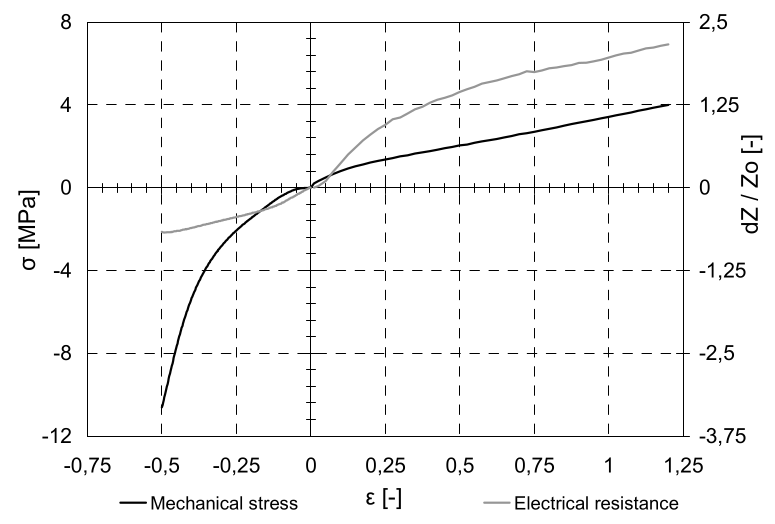
\includegraphics[width=\textwidth]{valentaConductiveRubber.png}
    \caption{Reproduced from \cite{valentaMechanicalElectricalTesting2008}, a summary of compression and tension effects on electrical properties for Elastosil\textsuperscript{\tiny\textregistered} R570/70 (Shore A 70) silicone.}
    \label{fg:conductiveRubber}
\end{figure}

Gallium-Indium Eutectic Alloys (eGaIn) have emerged as a potential deformable conductor. eGaIn is a family of alloys that contain gallium, indium and sometimes tin or other metals. One eGaIn formula is sometimes sold under the trade name Galinstan. A typical tin containing eutectic alloy such as Galinstan can have 68.5\% Ga, 21.5\% In and 10\% Sn \cite{liuCharacterizationNontoxicLiquidMetal2012}, while a typical alloy without tin can have 75\% Ga and 25\% In \cite{dickeyEutecticGalliumIndiumEGaIn2008}. Galinstan is reported to melt at as low as -19 \degree C \cite{surmannVoltammetricAnalysisUsing2005}, while others report that 75\% Ga 25\% In eGaIn melts at 15.5 \degree C \cite{dickeyEutecticGalliumIndiumEGaIn2008}. In either case, under most lab conditions eGaIn should be liquid.
Using liquid metal as a conductor means the surrounding body can undergo large deformations without large changes to material properties of the conductor. This is because the liquid will conform to the shape of the deformed cavity. Liquids also do not undergo strain hardening or fatigue. This means liquid metals can be better than solid metals in scenarios where they are expected to undergo large and repeated deformations, such as actuating soft robots.

eGaIn is advantageous among other liquid metals in that it has low toxicity \cite{dickeyEutecticGalliumIndiumEGaIn2008}, in contrast with mercury which is highly toxic. eGaIn is also stable under atmospheric conditions, compared to sodium-potassium alloy which is pyrophoric \cite{houghtonHazards2007}. eGaIn has negligible vapour pressure, meaning it will not vaporise under standard conditions. eGaIn does however form a solid oxide layer on contact with oxygen, which changes its properties on the material surface \cite{liuCharacterizationNontoxicLiquidMetal2012}.

75\% Ga 25\% In eGaIn  is reported to have electrical resistivity of $2.94\ \times10^{-7} \Omega m$ \cite{zrnicResistivitySurfaceTension1969}, which is about an order of magnitude higher than copper, commonly used as a solid conductor, and double that of stainless steel. This means that while eGaIn is a good conductor, circuits employing it will dissipate more heat and require more power input than equivalent solid circuits employing more conductive materials.

\section{Soft Robot Actuation}
\subsection{Externally Driven}
Most research soft robots require an external pressure source to drive actuation. For example, one such robot presented in \cite{morinCamouflageDisplaySoft2012} and pictured in Figure \ref{fg:conductiveRubber}, require an external pneumatic source through the silicone tubes in the back of the robot to move. The focus of these studies is on the actuators themselves, rather than on how to drive those actuators.

\begin{figure}[h!]
    \centering
    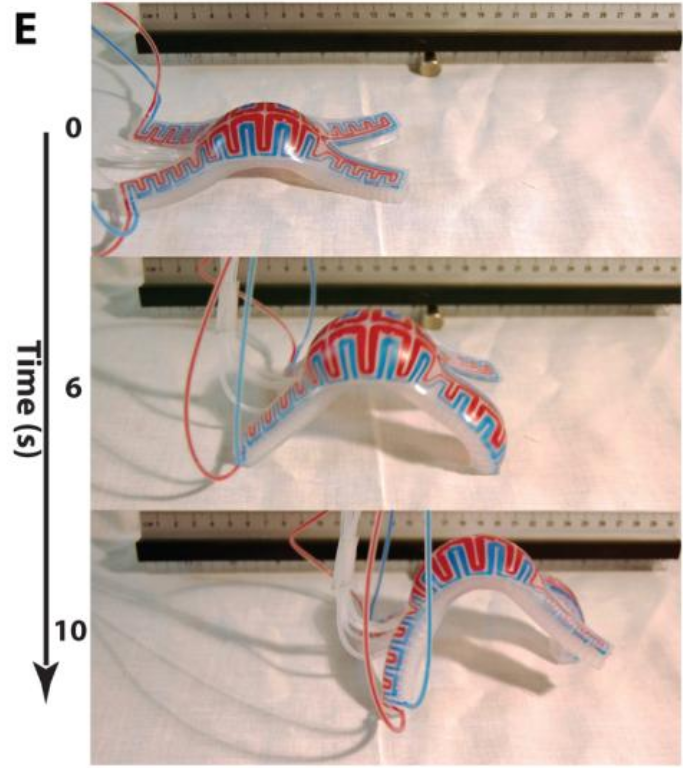
\includegraphics[width=0.5\textwidth]{externalpressure.png}
    \caption{Reproduced from \cite{morinCamouflageDisplaySoft2012}. The robot depicted requires external pressure sources supplied through tubes to move.}
    \label{fg:externalpressure}
\end{figure}

\subsection{Chemical}
A small proportion of research on soft robots suggested using chemical reactions to supply pressure for actuation. Kojimoto in \cite{kojimotoPneumaticBatteryChemical2012} described the use of a "pneumatic battery" composed of hydrogen peroxide that decomposes into water and oxygen gas. Shepard et al. demonstrated a different but similarly inventive solution that uses explosions to supply pressure in \cite{shepherdUsingExplosionsPower2013}. Figure \ref{fg:explosions} shows IR photos of the explosion-powered soft robot during activation. However, chemically powered soft robots are difficult to design and model due to the need to continuously replenish fuel and remove waste products. No chemically powered soft robot beyond the proof-of-concept stage was found.

\begin{figure}[h!]
    \centering
    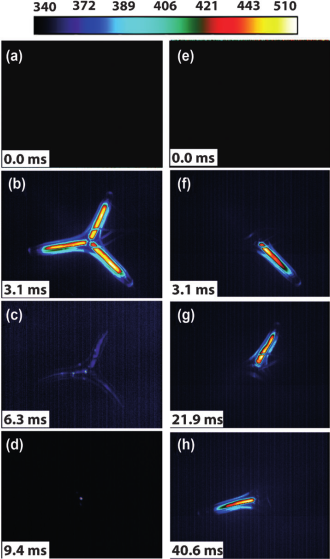
\includegraphics[width=0.3\textwidth]{explosions.png}
    \caption{IR photos reproduced from \cite{shepherdUsingExplosionsPower2013}. Images (a-d) shows simultaneous activation of all three chambers. Images (e-h) shows separate actuation with 15 ms delay between chambers. Temperature in \degree C.}
    \label{fg:explosions}
\end{figure}

\subsection{Electroactive Elastomer}
The third common type of soft robot was actuated using electroactive elastomers such as dielectric elastomers. Dielectric elastomers are constructed of an elastomer between two electrodes. Charging the electrodes can cause them to either attract or repeal each other, deforming the elastomer. A recent dielectric elastomer powered soft robot by Henke et al. \cite{henkeSoftDielectricElastomer2017} serves as a good example. In \cite{henkeSoftDielectricElastomer2017}, Henke et al. built an electronics-free biomimetic caterpillar robot that crawls and can be seen in Figure \ref{fg:catepillar}. A major challenge surrounding using electroactive elastomers in soft systems is that they cannot effectively actuate without a rigid "skeleton". Therefore, electroactive elastomers are suitable for wearable technologies and mixed systems, but not for fully deformable ones.

\begin{figure}[h!]
    \centering
    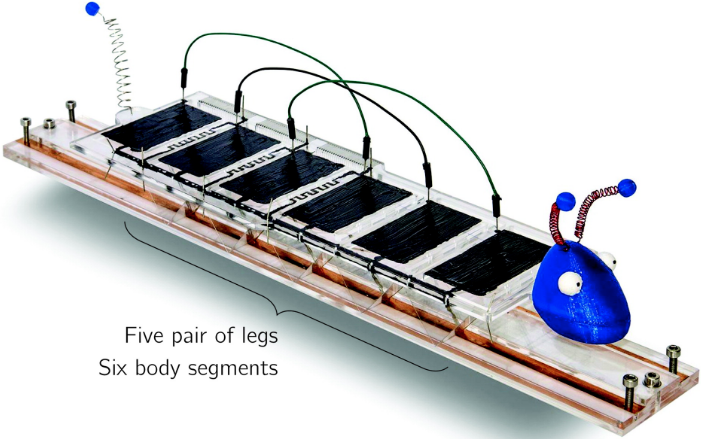
\includegraphics[width=0.3\textwidth]{catepillar.png}
    \caption{Image reproduced from \cite{henkeSoftDielectricElastomer2017}. "Trevor" the crawling caterpillar robot.}
    \label{fg:catepillar}
\end{figure}

\section{Electromagnetic Actuators}

\subsection{Electromagnetic Actuation using Liquid Metal}
There have only been a few examples that incorporated liquid metal into their electromagnetic actuator designs. All of them used some variety of eGaIn as their metal conductor and silicone to build the soft body.

Jin et al. pioneered this field with their 2015 paper that described the design, manufacture and testing of a stretchable loudspeaker \cite{jinStretchableLoudspeakerUsing2015}. The body of the loudspeaker was silicone while the voice coil was a spiral channel carved in the body and injected with eGaIn. Guo et al. extended on the work by Jin et al. with design and characterisation of mechanical actuators such as pincers and a swimming fish robot \cite{guoLiquidMetalSpiral2018}, both depicted in Figure \ref{fg:guoetal}. Both studies produced Lorentz force actuators using eGaIn voice coils and neodymium permanent magnets. Guo et al. used an airbrush spray gun to apply their liquid metal instead of the syringe and Scotch tape combination used by Jin et al. It is interesting that Guo et al. did not report any problems with oxidation of eGaIn, or any steps taken to limit oxygen contact, given they used an airbrush to apply the liquid metal which would mix the metal with air as it was being used.

\begin{figure}[h!]
    \centering
    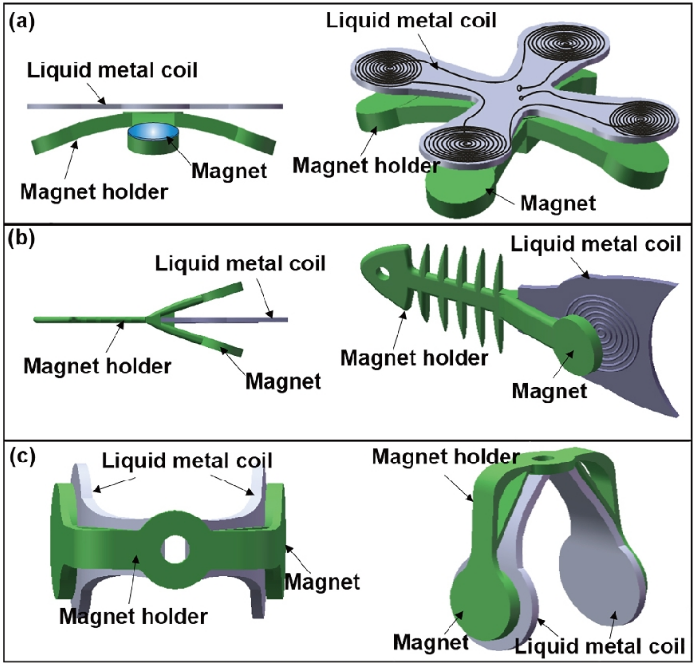
\includegraphics[width=0.5\textwidth]{guoetal.png}
    \caption{Reproduced from \cite{guoLiquidMetalSpiral2018}. Drawings of: (a) a jellyfish robot; (b) a fish robot; (c) a soft pincer.}
    \label{fg:guoetal}
\end{figure}

Do et al. took at different approach to Jin and Guo in their 2018 paper \cite{doMiniatureSoftElectromagnetic2018}. Instead of using microchannels in silicone, Do et al. injected eGaIn into silicone tubes which are then coiled. This study also included two example applications of their techniques, soft vibrotactile actuators (SVAs) and a miniature soft electromagnetic gripper (SEMG). A photo of the SVAs can be seen in Figure \ref{fg:guoetal}.

\begin{figure}[h!]
    \centering
    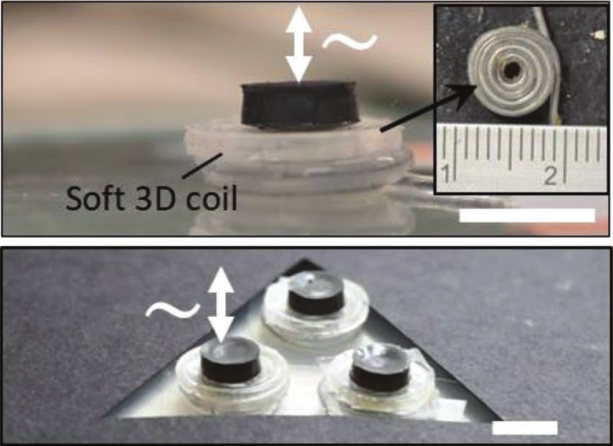
\includegraphics[width=0.5\textwidth]{doetal.png}
    \caption{Reproduced from \cite{doMiniatureSoftElectromagnetic2018}. Electromagnetic vibrotactile actuators using eGaIn.}
    \label{fg:guoetal}
\end{figure}

In the same study Do et al. also described the creation of a soft permanent magnet through mixing crushed neodymium magnet powder with liquid silicone and aligning poles while the silicone cures by placing the mould on a permanent magnet.

No study so far has explored creating soft counterparts to traditional electromagnetic motors, linear or rotational.

\subsection{Traditional Electromagnetic Motors}
Design and characterisation of stiff electromagnetic motors is a field that is comparatively mature, with a wealth of books and studies written on the subject such as \cite{moritzElectromechanicalMotionSystems2013}.

Linear voice coil motors are a type of motor that are relatively easy to construct and control. Linear voice coil motors produce movement via Lorentz force produced by interaction of a current carrying coil on a magnetic field produced by a permanent magnet. As shown in Figure \ref{fg:coilmotor}, there are two main configurations of linear voice coil motors: moving coil (left) and moving magnet (right)

\begin{figure}[h!]
    \centering
    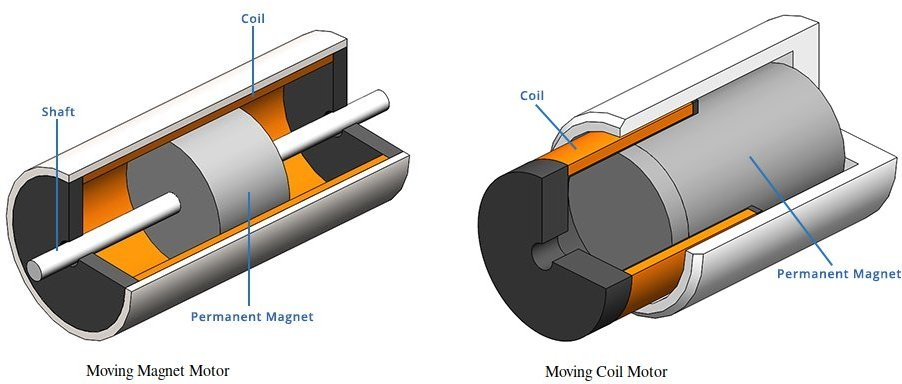
\includegraphics[width=\textwidth]{motorDiagram.jpg}
    \caption{Reproduced from \cite{h2wtechnologiesWhatVoiceCoil2018}. Simplified axisymmetric diagram of typical moving-wire voice coil motor.}
    \label{fg:coilmotor}
\end{figure}

As skeletal muscle can be approximated as a linear actuator, linear voice coil motors are also valuable for robot designs that seek to mimic biological function. A detailed guide on analytical modelling, optimisation and design strategies of linear direct-action motors by Ruddy and Hunter \cite{ruddyDesignOptimizationStrategies2011} is valuable especially for muscle-like linear motor design.

\subsection{Liquid Metal Electromagnetic Motors}
This literature review affirms the thus far overlooked opportunity to design, build and characterise an electromagnetic motor using liquid metal.

Such an electromagnetic motor will benefit from past research on liquid metal voice coil actuation in \cite{jinStretchableLoudspeakerUsing2015}, \cite{guoLiquidMetalSpiral2018} and \cite{doMiniatureSoftElectromagnetic2018}, especially their manufacturing methods. This approach to soft actuation also allows the transfer of research on rigid actuators such as \cite{ruddyDesignOptimizationStrategies2011}, rather than reinventing the wheel by designing other actuator modalities.

\section{Actuator Cooling}
Actuator heat exchange is a large challenge that bottlenecks the efficiency of some motor designs \cite{yoonEfficiencyIncreaseInduction2002}. Heat is more effectively removed from more accessible parts of the motor, but motor coils have the same rate of power dissipation, often causing a situation where the inside of a motor has a much higher temperature than the outside.

\subsection{Passive Heat Exchangers}
Passive heat exchangers include heat fins and other structures made from materials that are good conductors of heat and dimensions for large surface areas to dissipate heat. Passive devices are the simplest to design and implement, as there are no moving parts. However, it is very difficult to design passive exchange mechanisms that dissipate heat on the inside of a motor as well as on the outside.

\subsection{Liquid Heat Exchangers}
Liquid heat exchangers circulate a coolant through the actuator, and then the coolant is cooled externally. This approach creates the added complication of incorporating hydraulic channels into the motor coil design. Several recent innovations have been made to address this issue, explained in \cite{henkeChallengesOpportunitiesVery2018}. One new method involves manufacturing channels into the coil wire, through which liquid coolant is circulated \cite{wohlersDesignDirectLiquid2018}. This requires advanced manufacturing techniques and is not accessible for use in soft robots.

\begin{figure}[h!]
    \centering
    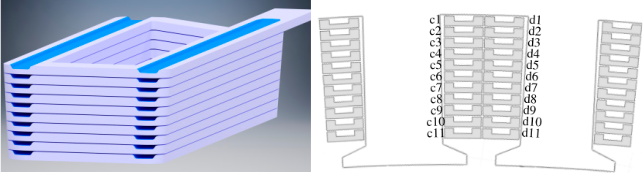
\includegraphics[width=\textwidth]{liquidcool.png}
    \caption{Reproduced from \cite{wohlersDesignDirectLiquid2018}. Left: illustration of 3D cast coil. Right: schematic model of 3D casted coil.}
    \label{fg:coilmotor}
\end{figure}

\subsection{Superconductors}
Other methods include using liquid helium\cite{hoenigDenseSupercriticalheliumCooled1975}, liquid nitrogen or liquid neon\cite{henkeChallengesOpportunitiesVery2018} to create superconductors, where heating due to wire resistance is not an issue. This again creates conditions and constraints, especially the extremely low temperature, that are not acceptable for most design requirements.

\subsection{Liquid Metal Circulation}
There is an evident opportunity for heat exchange via circulating the actual conductors. eGaIn has a specific heat capacity of 296 $J\cdot (kg\cdot K)^{-1}$ \cite{hodesPotentialGalinstanBasedMinichannel2014}, which is lower than water, but higher than other liquid metals such as mercury. eGaIn also has good thermal conductivity at 16.5 $W\cdot(m\cdot K)^{-1}$, which is again higher than mercury but lower than other materials used as conductors such as copper \cite{naveThermalConductivity2019}.

\newpage

\section{Statement of Research Intent}

\subsection{Motivation and Purpose}

To design, build and characterise an electromagnetic motor that uses liquid metal coils and can circulate metal in its coils.

\subsection{Aims and Milestones}

The aim by the end of this project is to have an operational motor that uses liquid metal as its coil conductor.

The motor should:
\begin{itemize}
    \item Output enough force to drive a fluid pump. This force was determined as 9 N after liaising with the Liquid Metal Pump project.
    \item Dissipate heat well enough while driving the fluid pump that it does not fail due to overheating
    \item Be well characterised in terms of current, power and mass efficiency.
\end{itemize}

This project has five major milestones, modelling, design, part and tool construction, assembly and characterisation.

The first milestone is to develop the mathematical model of an electromagnetic motor that uses liquid metal in its coils.

The second milestone is to establish design requirements, and use optimisation to find the most efficient motor within those design requirements.

Parts and tools will then need to be drafted and made. Completed parts and tools ready for assembly will be another milestone.

The next milestone is to assemble all the parts together to form an operational motor.

Once there is an operational motor, the final milestone is to conclude testing on the motor to characterise its properties.

\subsection{Method}
A voice coil motor will be used as the base design due to simple coil arrangement that allows for easiest winding of silicone tube. Voice coil motors are also generally simple in design and construction, requiring few parts in total and a singular moving part.

A mathematical model of a voice coil motor that uses eGaIn coils will then be created. There is a large existing corpus on how linear voice coil motors are designed, but most appear in old and specialised publications.

Design requirements will then be set based on equipment, resource and safety constraints. The mathematical model will then be used to optimise design dimensions to produce the highest efficiency motor within design requirements.

With the design dimensions, the specifics of components and assembly will be designed. All parts will be drafted in CAD software and have engineering drawings made. The assembly plan will follow safety precautions against known hazards.

Motor components and tools for assembly will then be manufactured. These parts will be made using available equipment in the workshop, including a lathe, a mill, a laser cutter, hand tools and a SLA 3D printer.

The components will then be assembled following the assembly plan, using tools made to assist assembly.

The assembled motor will finally be characterised using an experiment that measures the force output of the motor as current input changes.

\newpage

\printbibliography

\end{document}
